\documentclass[aspectratio=169, 10pt]{beamer}
\usetheme{Madrid}
\usecolortheme{whale}
\setbeamertemplate{blocks}[rounded][shadow=false]

% Remove clutter navigation symbols
\setbeamertemplate{navigation symbols}{}

\usepackage{graphicx}
\usepackage{booktabs}
\usepackage{amsmath}
\usepackage{xcolor}

\graphicspath{{reports/figures/}{./}}

% Custom Colors
\definecolor{iitgblue}{RGB}{20, 45, 85}
\definecolor{accentorange}{RGB}{217, 95, 2}
\definecolor{tealgreen}{RGB}{27, 158, 119}
\setbeamercolor{palette primary}{bg=iitgblue, fg=white}
\setbeamercolor{structure}{fg=iitgblue}

\title[Monsoon Sentinel (Part 1)]{Monsoon Sentinel (Part 1): Embedded Sensor Interfacing, Resilient Telemetry, and Physical Dataset Acquisition}
\subtitle{Term Project Presentation --- BSc (Hons) in Data Science \& AI}
\author[Ganesha Nischal Sai]{Ganesha Nischal Sai \\ \small Roll Number: 230323010}
\institute[IIT Guwahati]{Indian Institute of Technology Guwahati}
\date{November 2026}

\begin{document}

% ==========================================================
% SLIDE 1: Title / Thumbnail Slide (IITG Requirement)
% ==========================================================
\begin{frame}[plain]
    \IfFileExists{Thumbnail_IITG.png}{%
        \centering
        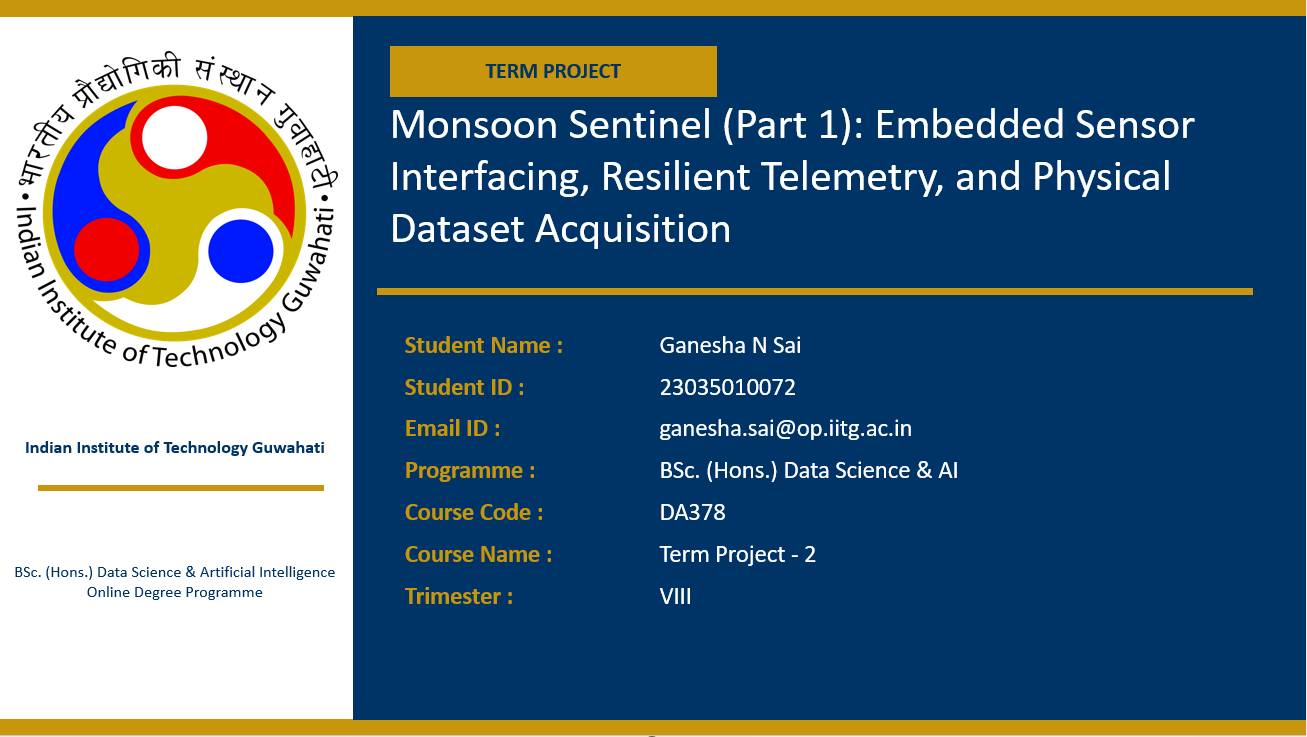
\includegraphics[width=\textwidth, height=\textheight, keepaspectratio]{Thumbnail_IITG.png}%
    }{%
        \titlepage
    }
\end{frame}

% ==========================================================
% SLIDE 2: Self-Introduction & Project Scope
% ==========================================================
\begin{frame}{Introduction \& Project Scope}
    \begin{columns}[T]
        \begin{column}{0.58\textwidth}
            \textbf{Presenter Profile:}
            \begin{itemize}
                \item \textbf{Name:} Ganesha Nischal Sai
                \item \textbf{Programme:} BSc (Hons) Data Science \& AI, IIT Guwahati
                \item \textbf{Submission:} Term Project (Part 1 of 2)
            \end{itemize}
            \vspace{0.4cm}
            \textbf{Project 1 vs. Project 2 Split:}
            \begin{itemize}
                \item \textbf{Part 1 (Current):} Sensor interfacing, 100\,Hz telemetry driver, $I^2\text{C}$ bus fault recovery, host ingestion, and physical dataset collection.
                \item \textbf{Part 2 (Next Stage):} CMSIS-DSP accelerated spectral transforms, group-stratified ML benchmarks, and TinyML on-device inference.
            \end{itemize}
        \end{column}
        \begin{column}{0.38\textwidth}
            \begin{alertblock}{Core Objective}
                Eliminate synthetic data reliance by constructing a real cyber-physical sensor rig to capture verified, uncorrupted kinetic motion regimes.
            \end{alertblock}
            \vspace{0.2cm}
            \begin{block}{Hardware Acquired}
                \begin{itemize}
                    \item STM32 Nucleo-F401RE
                    \item MPU-6050 6-DOF IMU
                    \item nanoDLA Logic Analyzer
                \end{itemize}
            \end{block}
        \end{column}
    \end{columns}
\end{frame}

% ==========================================================
% SLIDE 3: Problem Statement & Motivation
% ==========================================================
\begin{frame}{Problem Statement \& Embedded Challenges}
    \textbf{The Challenge: Acquiring High-Cadence Kinetic Telemetry}
    \begin{itemize}
        \item Continuous spectral analysis (FFT, swell energy) requires an uninterrupted, low-jitter sampling rate (100\,Hz).
        \item Edge sensors in remote maritime and mast environments suffer from silent failures:
    \end{itemize}
    \vspace{0.2cm}
    \begin{columns}[T]
        \begin{column}{0.48\textwidth}
            \begin{block}{Hardware Failure Modes}
                \begin{itemize}
                    \item \textbf{$I^2\text{C}$ Slave Line-Clamping:} Slave latches SDA low during transient glitches; freezes entire bus.
                    \item \textbf{Synchronous I/O Stalls:} Blocking HAL calls choke CPU headroom.
                    \item \textbf{Serial Ingestion Overruns:} OS disk write latency drops incoming packets.
                \end{itemize}
            \end{block}
        \end{column}
        \begin{column}{0.48\textwidth}
            \begin{exampleblock}{Part 1 Engineering Solutions}
                \begin{itemize}
                    \item \textbf{9-Clock Bus Recovery:} Firmware bit-bang routine unclamps stuck slave shift registers.
                    \item \textbf{Threaded Ingestion:} Producer-consumer architecture decouples UART from disk.
                    \item \textbf{Automated Test Suite:} 12 unit tests verify temporal and spectral determinism.
                \end{itemize}
            \end{exampleblock}
        \end{column}
    \end{columns}
\end{frame}

% ==========================================================
% SLIDE 4: Physical Testbed & Hardware Setup
% ==========================================================
\begin{frame}{Physical Testbed \& Hardware Setup}
    \begin{columns}[T]
        \begin{column}{0.52\textwidth}
            \textbf{Compute Core \& Sensor Node:}
            \begin{itemize}
                \item \textbf{MCU:} STM32 Nucleo-F401RE (ARM Cortex-M4F @ 84\,MHz, 512\,KB Flash, 96\,KB SRAM).
                \item \textbf{IMU:} InvenSense MPU-6050 (3-axis Accel $\pm 2g$, 3-axis Gyro $\pm 250^\circ/\text{s}$).
                \item \textbf{Bus:} $I^2\text{C}1$ on PB8 (SCL) and PB9 (SDA) @ 100\,kHz.
                \item \textbf{UART Telemetry:} USART2 (PA2/PA3) @ 115,200\,baud.
                \item \textbf{Logic Analyzer:} nanoDLA 24\,MHz tapping I2C and UART pins to verify frame timing and ACKs.
            \end{itemize}
            \vspace{0.2cm}
        \end{column}
        \begin{column}{0.45\textwidth}
            \IfFileExists{tabletop.png}{%
                \centering
                \includegraphics[width=\textwidth, height=0.42\textheight, keepaspectratio]{tabletop.png}\\
                \vspace{0.1cm}
                \scriptsize \textbf{Figure:} Benchtop Testbed Assembly
            }{%
                \begin{block}{Benchtop Testbed}
                    Nucleo-F401RE + Breadboard + MPU-6050 + logic analyzer tap harness connected to workstation.
                \end{block}
            }
            \vspace{0.2cm}
            \IfFileExists{stm32_pinout.png}{%
                \centering
                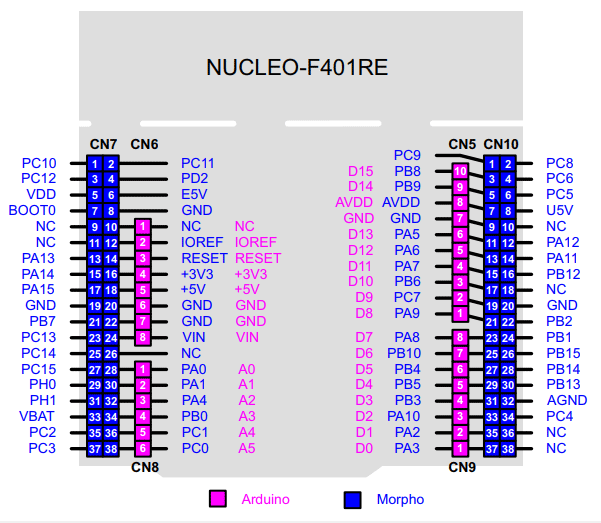
\includegraphics[width=0.85\textwidth, height=0.35\textheight, keepaspectratio]{stm32_pinout.png}
            }{%
                \scriptsize PB8: SCL $|$ PB9: SDA $|$ PA2: TX $|$ PA3: RX
            }
        \end{column}
    \end{columns}
\end{frame}

% ==========================================================
% SLIDE 5: Mechanical Cantilever Surrogate & Regimes
% ==========================================================
\begin{frame}{Mechanical Cantilever Surrogate Rig}
    \begin{columns}[T]
        \begin{column}{0.5\textwidth}
            \textbf{Physical Excitation Surrogate:}
            \begin{itemize}
                \item Flexible 30\,cm ruler cantilever clamped to the test bench with MPU-6050 mounted at tip.
                \item Emulates spar-buoy structural flexure, mast aero-buffeting, and vortex shedding.
            \end{itemize}
            \vspace{0.2cm}
            \textbf{5 Synthesized Motion Regimes:}
            \begin{enumerate}
                \item \textbf{Nominal Baseline:} Calm station-keeping.
                \item \textbf{Structural Tilt:} Static angular list ($0^\circ$--$55^\circ$).
                \item \textbf{Acoustic Vibration:} 400\,Hz motor/acoustic excitation.
                \item \textbf{Impulse Shock:} Mechanical taps and impacts.
                \item \textbf{Mast Buffeting:} Continuous airflow excitation.
            \end{enumerate}
        \end{column}
        \begin{column}{0.46\textwidth}
            \IfFileExists{fan_ruler.png}{%
                \centering
                \includegraphics[width=\textwidth, height=0.72\textheight, keepaspectratio]{fan_ruler.png}\\
                \scriptsize \textbf{Figure:} Fan \& Cantilever Ruler Testbed
            }{%
                \begin{block}{Surrogate Testbed Setup}
                    Fan air stream directed face-on at ruler tip to excite natural bending modes.
                \end{block}
            }
        \end{column}
    \end{columns}
\end{frame}

% ==========================================================
% SLIDE 6: Firmware Architecture & Latency Budget
% ==========================================================
\begin{frame}{Firmware Architecture \& Execution Budget}
    \textbf{100\,Hz Deterministic Sampling Loop (main.c):}
    \begin{itemize}
        \item Timing enforced by non-cumulative SysTick polling ($\Delta t \ge 10\,\text{ms}$).
        \item 14-byte burst read across $I^2\text{C}$ retrieves Accel, Temp, and Gyro data simultaneously.
    \end{itemize}
    \vspace{0.1cm}
    \begin{table}[h]
        \centering
        \scriptsize
        \begin{tabular}{llccc}
            \toprule
            \textbf{Pipeline Operation} & \textbf{Peripheral Mode} & \textbf{Duration (ms)} & \textbf{CPU Cycles} & \textbf{Core Load (\%)} \\
            \midrule
            $I^2\text{C}$ Burst Read (14\,B) & Synchronous Polling (100\,kHz) & 1.500 & 126,000 & 15.00\% \\
            ASCII Formatting & In-Memory (\texttt{sprintf}) & 0.008 & 672 & 0.08\% \\
            UART Telemetry TX ($\sim$40\,B) & Synchronous Polling (115.2\,kbaud) & 3.472 & 291,648 & 34.72\% \\
            \midrule
            \textbf{Total Blocking Wait} & \textbf{Synchronous Wait} & \textbf{4.980} & \textbf{418,320} & \textbf{49.80\%} \\
            SysTick Polling Idle Budget & Main Loop Margin & 5.020 & 421,680 & 50.20\% \\
            \midrule
            \textbf{Available Period} & \textbf{100\,Hz Period ($T_s = 10$\,ms)} & \textbf{10.000} & \textbf{840,000} & \textbf{100.00\%} \\
            \bottomrule
        \end{tabular}
    \end{table}
    \vspace{0.1cm}
    \begin{alertblock}{Key Finding}
        Synchronous I/O blocks the MCU core for 49.8\% of each cycle. This cycle-accurate audit establishes the requirement for DMA-driven pipelines in Part 2.
    \end{alertblock}
\end{frame}

% ==========================================================
% SLIDE 7: Resilient Logging & Host Ingestion
% ==========================================================
\begin{frame}{Host Ingestion \& $I^2\text{C}$ Bus Recovery}
    \begin{columns}[T]
        \begin{column}{0.5\textwidth}
            \textbf{1. Algorithmic $I^2\text{C}$ Bus Recovery:}
            \begin{itemize}
                \item \textbf{Failure Mode:} Slave holds SDA low after glitch.
                \item \textbf{Recovery Routine:}
                \begin{enumerate}
                    \item Disable $I^2\text{C}$ clock.
                    \item Switch PB8/PB9 to Open-Drain GPIO.
                    \item Toggle SCL 9 times manually (100\,kHz) to clock out hung slave shift register.
                    \item Issue manual STOP condition.
                    \item Re-initialize $I^2\text{C}1$.
                \end{enumerate}
            \end{itemize}
            \vspace{0.2cm}
            \textbf{2. Multi-Threaded Host Ingestion:}
            \begin{itemize}
                \item Producer thread reads serial frames into an in-memory queue (\texttt{queue.Queue}).
                \item Consumer thread handles CSV disk writing.
            \end{itemize}
        \end{column}
        \begin{column}{0.46\textwidth}
            \IfFileExists{screen_data.png}{%
                \centering
                \includegraphics[width=\textwidth, height=0.65\textheight, keepaspectratio]{screen_data.png}\\
                \scriptsize \textbf{Figure:} Live Serial Telemetry Streaming
            }{%
                \begin{block}{Live Serial Stream}
                    Continuous ASCII stream: \texttt{timestamp,ax,ay,az,gx,gy,gz} @ 100\,Hz.
                \end{block}
            }
            \vspace{0.1cm}
        \end{column}
    \end{columns}
\end{frame}

% ==========================================================
% SLIDE 8: Dataset Registry & Motion Partitioning
% ==========================================================
\begin{frame}{Dataset Registry \& Motion Partitioning}
    \textbf{Curated Physical Dataset (100\,Hz, $N=128$, Step=64):}
    \begin{table}[h]
        \centering
        \small
        \begin{tabular}{clrcccc}
            \toprule
            \textbf{ID} & \textbf{Regime Name} & \textbf{Raw Files} & \textbf{Total Windows} & \textbf{Duration (s)} & \textbf{Class Share} \\
            \midrule
            0 & Nominal\_Baseline   & 10 & 7,680  & 4,923.55 & 62.20\% \\
            1 & Structural\_Tilt    &  3 & 1,422  &   913.30 & 11.52\% \\
            2 & Acoustic\_Vibration &  2 &   378  &   243.67 &  3.06\% \\
            3 & Impulse\_Shock      &  1 &   189  &   121.74 &  1.53\% \\
            4 & Mast\_Buffeting     &  6 & 2,679  & 1,720.19 & 21.70\% \\
            \midrule
            \textbf{--} & \textbf{Total Verified} & \textbf{22} & \textbf{12,348} & \textbf{7,922.45} & \textbf{100.00\%} \\
            \bottomrule
        \end{tabular}
    \end{table}
    \vspace{0.2cm}
    \begin{columns}[T]
        \begin{column}{0.48\textwidth}
            \begin{block}{Scale \& Scope}
                \begin{itemize}
                    \item 2.20 hours of continuous physical logging.
                    \item 12,348 sliding windows of 1.28\,s each (50\% overlap).
                \end{itemize}
            \end{block}
        \end{column}
        \begin{column}{0.48\textwidth}
            \begin{exampleblock}{Dataset Cleansing Highlight}
                Recovered \texttt{Xaxis\_FAN\_Ceiling.csv} by identifying single 430\,s startup pause and restoring 307 clean windows.
            \end{exampleblock}
        \end{column}
    \end{columns}
\end{frame}

% ==========================================================
% SLIDE 9: Automated 12-Test Validation Suite
% ==========================================================
\begin{frame}{Automated 12-Test Ingestion Validation Suite}
    \textbf{Reproducibility Test Harness (\texttt{tests/test\_part1\_telemetry\_pipeline.py}):}
    \begin{columns}[T]
        \begin{column}{0.5\textwidth}
            \begin{itemize}
                \item \textbf{TC-01 (Cadence):} $\overline{\Delta t} = 10.0 \pm 0.1\,\text{ms}$ \hfill \textcolor{tealgreen}{\textbf{[PASS]}}
                \item \textbf{TC-02 (Jitter):} $\sigma_{\Delta t} < 0.5\,\text{ms}$ \hfill \textcolor{tealgreen}{\textbf{[PASS]}}
                \item \textbf{TC-03 (Continuity):} $\Delta t \le 20.0\,\text{ms}$ (0 dropped) \hfill \textcolor{tealgreen}{\textbf{[PASS]}}
                \item \textbf{TC-04 (Stale Guard):} Repeated frames $< 20$ \hfill \textcolor{tealgreen}{\textbf{[PASS]}}
                \item \textbf{TC-05 (Accel Range):} No saturation ($\pm 32767$) \hfill \textcolor{tealgreen}{\textbf{[PASS]}}
                \item \textbf{TC-06 (Gyro Range):} No saturation ($\pm 32767$) \hfill \textcolor{tealgreen}{\textbf{[PASS]}}
            \end{itemize}
        \end{column}
        \begin{column}{0.5\textwidth}
            \begin{itemize}
                \item \textbf{TC-07 (Gravity Norm):} $1.00 \pm 0.08\,g$ \hfill \textcolor{tealgreen}{\textbf{[PASS]}}
                \item \textbf{TC-08 (Noise Floor):} Stationary $\le 0.010\,g$ \hfill \textcolor{tealgreen}{\textbf{[PASS]}}
                \item \textbf{TC-09 (Gyro Bias):} Offset $\le 3.0^\circ/\text{s}$ \hfill \textcolor{tealgreen}{\textbf{[PASS]}}
                \item \textbf{TC-10 (Integrity):} 0 NaNs and 0 Infs in v4 \hfill \textcolor{tealgreen}{\textbf{[PASS]}}
                \item \textbf{TC-11 (Nyquist):} $\Delta f = 0.78125$\,Hz, $f_{max} = 50$\,Hz \hfill \textcolor{tealgreen}{\textbf{[PASS]}}
                \item \textbf{TC-12 (Parseval):} Band energy $\sum = E_{total}$ \hfill \textcolor{tealgreen}{\textbf{[PASS]}}
            \end{itemize}
        \end{column}
    \end{columns}
    \vspace{0.3cm}
    \begin{alertblock}{Validation Outcome}
        \textbf{Result: 12 passed in 2.55s} via pytest. Proves zero frame loss, clock stability, and strict physical scaling.
    \end{alertblock}
\end{frame}

% ==========================================================
% SLIDE 10: Exploratory Data Analysis & Physical Insights
% ==========================================================
\begin{frame}{Exploratory Data Analysis \& Separability}
    \IfFileExists{eda_scatter_separability.png}{%
        \centering
        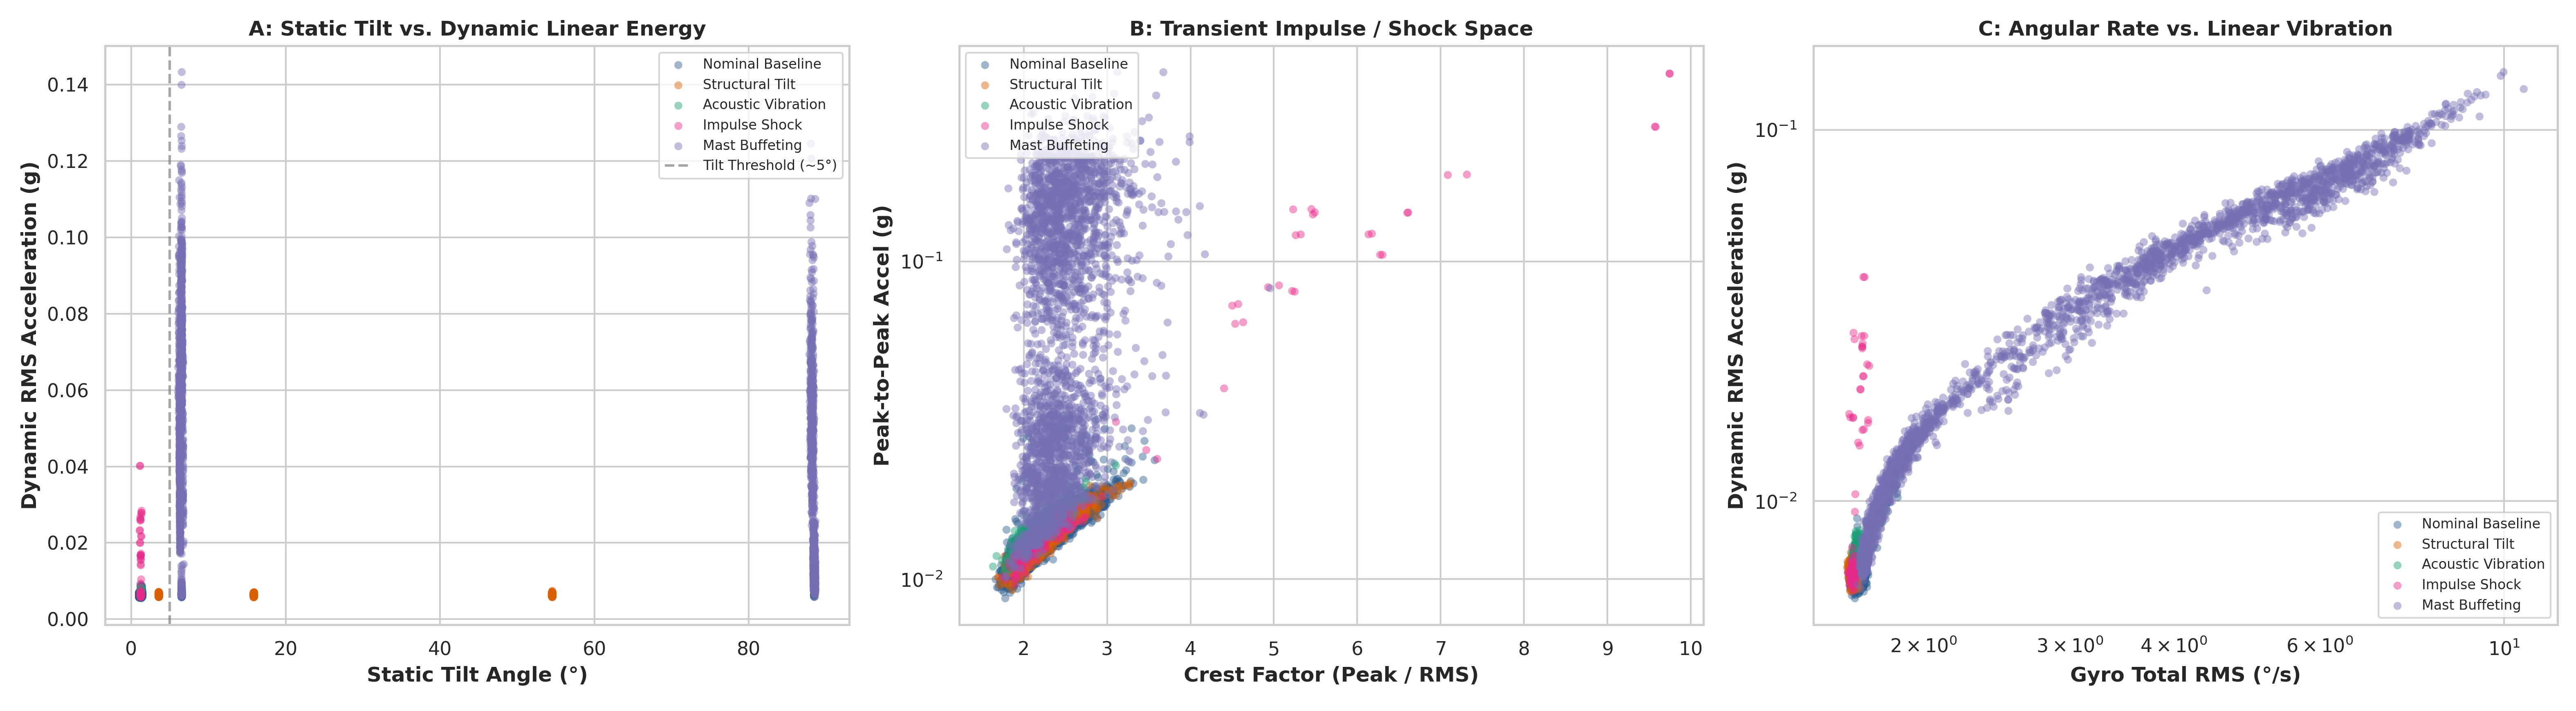
\includegraphics[width=0.98\textwidth, height=0.55\textheight, keepaspectratio]{eda_scatter_separability.png}
    }{%
        \begin{block}{Feature Separability}
            Panel A: Tilt vs RMS $|$ Panel B: Peak-to-Peak vs Crest Factor $|$ Panel C: Gyro vs Linear RMS
        \end{block}
    }
    \vspace{0.1cm}
    \begin{columns}[T]
        \begin{column}{0.32\textwidth}
            \textbf{1. Structural Tilt:}
            $\text{Tilt} = 24.7^\circ \pm 21.7^\circ$ while dynamic energy remains at noise floor ($0.0064\,g$).
        \end{column}
        \begin{column}{0.32\textwidth}
            \textbf{2. Impulse Shock:}
            Crest Factor shoots to $2.81 \pm 1.53$ (peak 9.74) with large peak-to-peak excursions ($0.032\,g$).
        \end{column}
        \begin{column}{0.32\textwidth}
            \textbf{3. Mast Buffeting:}
            Dynamic RMS surges $5.6\times$ ($0.0365\,g$), gyro doubles, and $f_{dom}$ drops to 11.31\,Hz resonance.
        \end{column}
    \end{columns}
\end{frame}

% ==========================================================
% SLIDE 11: Discussion & Hardware Boundaries
% ==========================================================
\begin{frame}{Discussion: Key Insights \& Technical Boundaries}
    \begin{columns}[T]
        \begin{column}{0.48\textwidth}
            \begin{block}{Physical Separability Confirmed}
                \begin{itemize}
                    \item \textbf{Cantilever Bending Resonance:} The dominant frequency shift from 25.59\,Hz (white noise) to 11.31\,Hz proves FFT captures real structural physics.
                    \item \textbf{Orientation Invariance:} Norm computation $\|\vec{a} - \bar{\vec{a}}\|$ successfully decouples dynamic agitation from static gravity tilt.
                \end{itemize}
            \end{block}
        \end{column}
        \begin{column}{0.48\textwidth}
            \begin{alertblock}{The 400\,Hz Acoustic Boundary}
                \begin{itemize}
                    \item \textbf{Observation:} 400\,Hz Acoustic Vibration yielded RMS of $0.0072\,g$, nearly identical to baseline ($0.0065\,g$).
                    \item \textbf{Root Cause:} Sampling rate of 100\,Hz imposes a 50\,Hz Nyquist limit; sensor low-pass filter suppresses acoustic frequencies.
                    \item \textbf{Design Justification:} Establishes physical need for I2S MEMS microphone (INMP441) in future revisions.
                \end{itemize}
            \end{alertblock}
        \end{column}
    \end{columns}
\end{frame}

% ==========================================================
% SLIDE 12: Summary & Roadmap to Part 2
% ==========================================================
\begin{frame}{Summary \& Roadmap to Part 2}
    \begin{columns}[T]
        \begin{column}{0.48\textwidth}
            \textbf{Part 1 Deliverables Completed:}
            \begin{itemize}
                \item Bare-metal STM32F401RE $I^2\text{C}$/UART acquisition driver.
                \item 9-clock $I^2\text{C}$ bus lockup recovery routine.
                \item Multi-threaded host serial logging engine.
                \item 12-test automated ingestion validation suite.
                \item 12,348 verified feature vectors across 22 sessions.
            \end{itemize}
        \end{column}
        \begin{column}{0.48\textwidth}
            \textbf{Part 2 Roadmap (Edge TinyML):}
            \begin{itemize}
                \item \textbf{CMSIS-DSP Integration:} Linking \texttt{arm\_rfft\_fast\_f32} on Cortex-M4F hardware FPU.
                \item \textbf{Group-Stratified ML:} Leak-free cross-validation across \texttt{source\_file} groups.
                \item \textbf{On-Device Classification:} Linear SVM, Random Forest, and Quantized MLP deployed in C.
                \item \textbf{Bandwidth Savings:} 99.9\% reduction in telemetry bandwidth.
            \end{itemize}
        \end{column}
    \end{columns}
    \vspace{0.4cm}
    \begin{center}
        \textbf{\large Thank You!} \\[0.2cm]
    \end{center}
\end{frame}

\end{document}